\begin{figure}
  \centering
  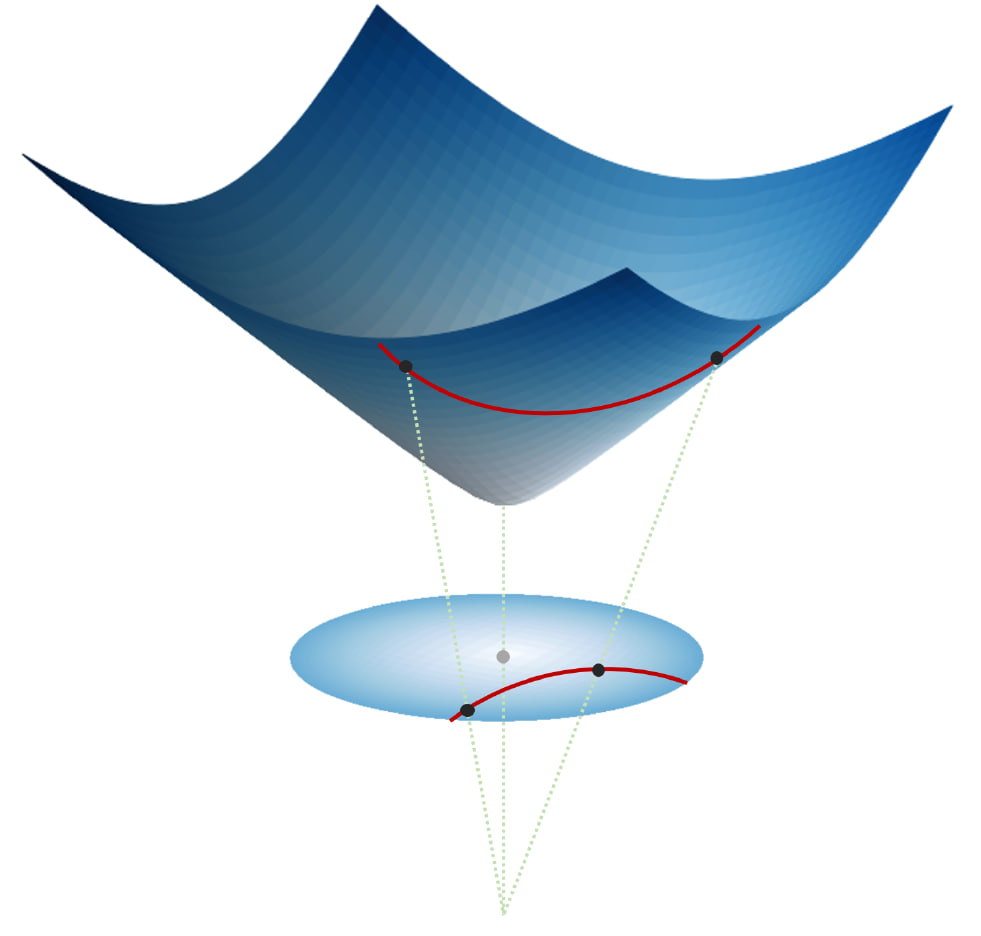
\includegraphics[width=0.5\textwidth]{figs/hyperboloidToPoincare.jpg}

    % \begin{tikzpicture}
    %     \begin{axis}[view={30}{20},axis lines=none]
    %       % Draw the hyperboloid
    %       \addplot3[surf, shader=interp, colormap/blackwhite, domain=-2:2]
    %         {x^2+y^2+1};
        
    %     % Limit geodesic curve to fit within the drawn hyperboloid
    %     \addplot3[domain=-0.9:1.63,samples=50, samples y=0, thick, blue]
    %     {sqrt(sinh(x)^2 + cosh(x)^2 + 1)+1};

        
          
    %     \end{axis}


    %   \end{tikzpicture}
  \caption{Illustration of the hyperboloid (top) and its connection to the Poincaré disk (bottom)\cite{Chami2021representationLearningAlgorithmsHyperbolicSpaces}.}
  \label{fig:hyperboloidToPoincareBall}
\end{figure}